\chapter{PandaX-III项目介绍}
\label{chapter:intro}
%\pkuthssffaq % 中文测试文字。

正如上文所说,NLDBD 是一种极其稀有的事件,既有实验已经给出它的半衰期 $T^{0\nu}_{1/2}>1.07\times10^{26}$ 年。如果要由此计算出中微子质量顺序,那么至少需要 1 吨量级的衰变元素才有能达成该目标。所以 NLDBD 的相关实验需要解决以下难点:

\vspace{0.4cm}
\begin{enumerate}
    \item 顺利制造和生产出 1 吨以上有可能发生NLDBD事件的放射性元素。
    \item 建造出具有极佳的能量分辨率和位置分辨率的探测器,达到 NLDBD 事件探测的需求。
    \item 探测器本底噪声很低,在灵敏区域内的背景事件数目应小于 $10^{-4}$ \ckky。
    \item 寻找到高效区分 NLDBD 信号及背景事件的方法。
\end{enumerate}
\vspace{0.4cm}

本章节简单介绍了PandaX-III实验如何通过适当选择衰变元素及合理设计探测器结构等操作来解决上述困难,以够顺利达成探测 NLDBD 事件的实验目标。

\section{元素选择}

在诸多可以发生 NLDBD 事件的放射性元素中,\xeots 在自然界中同位素丰度较高,价格相对便宜,自身还可以作为气体探测器的工作气体,因此 PandaX-III 选取了它作为目标衰变元素。\xeots NLDBD 事件释放出的总能量为 $Q_{\beta\beta}=2458$keV,这个能量相对较高,能够避开部分低能背景辐射。但是在 $Q_{\beta\beta}$ 附近, $^{214}$Bi 和 $^{208}$Tl 两种元素的 $\gamma$ 衰变可能会对实验造成影响,其中 $^{214}$Bi 释放出的 $\gamma$ 射线能量为 2448keV,只比 $Q_{\beta\beta}$ 低10keV 左右。更为严重的是,这两种元素是 $^{238}$U 和 $^{232}$Th 衰变链的中间产物,他们广泛存在于生产生活中的各种材料中,因此降低探测器材料中 \utte 和 \thttt 对实验的影响是 PandaX-III 所面临的一个巨大挑战。

PandaX-III 使用了 10bar 的高压气氙作为探测气体,其中 \xeots 的丰度为 90\%。为了配合电子学读出系统并增强读出信号的质量,探测气体同时混合了 1\% 的 TMA(trimethylamine)。根据 NEXT 实验的相关研究,使用这种混合气体作为探测介质能够在 $Q_{\beta\beta}$ 处达到 3\% 的能量分辨率\supercite{azevedoh2015accurate}。

\section{探测器构造}
\label{section:detector}

PandaX-III 计划建造 5 个 200kg 级高压气氙时间漂移室(Time Projection Chamber, TPC)用于探测 NLDBD 事件,探测器结构如图\ref{fig:detector}左所示。高压气体TPC的相关技术在上个世纪 90 年代便已经成熟,它的能量分辨率远远优于液体TPC。如果使用直接采集电离电子的读取器件作为探测器读出系统,高压气体TPC的能量分辨率能够达到液体的10倍。高压气体TPC另外一个巨大的优势是它具有优秀的位置分辨本领,配合像素或者条状读出可以十分便捷的重建出事件的径迹。在寻找 NLDBD 的相关试验中,径迹信息可以用与高效的鉴别本底背景和 NLDBD 信号,从而可以极大的压低背景噪声,以满足实验极低本底的需求。本文第\ref{chapter:cnn}章着重介绍了使用深度卷积神经网络进行背景及信号鉴别的方法。

\begin{figure}[tbp]
    \centering
    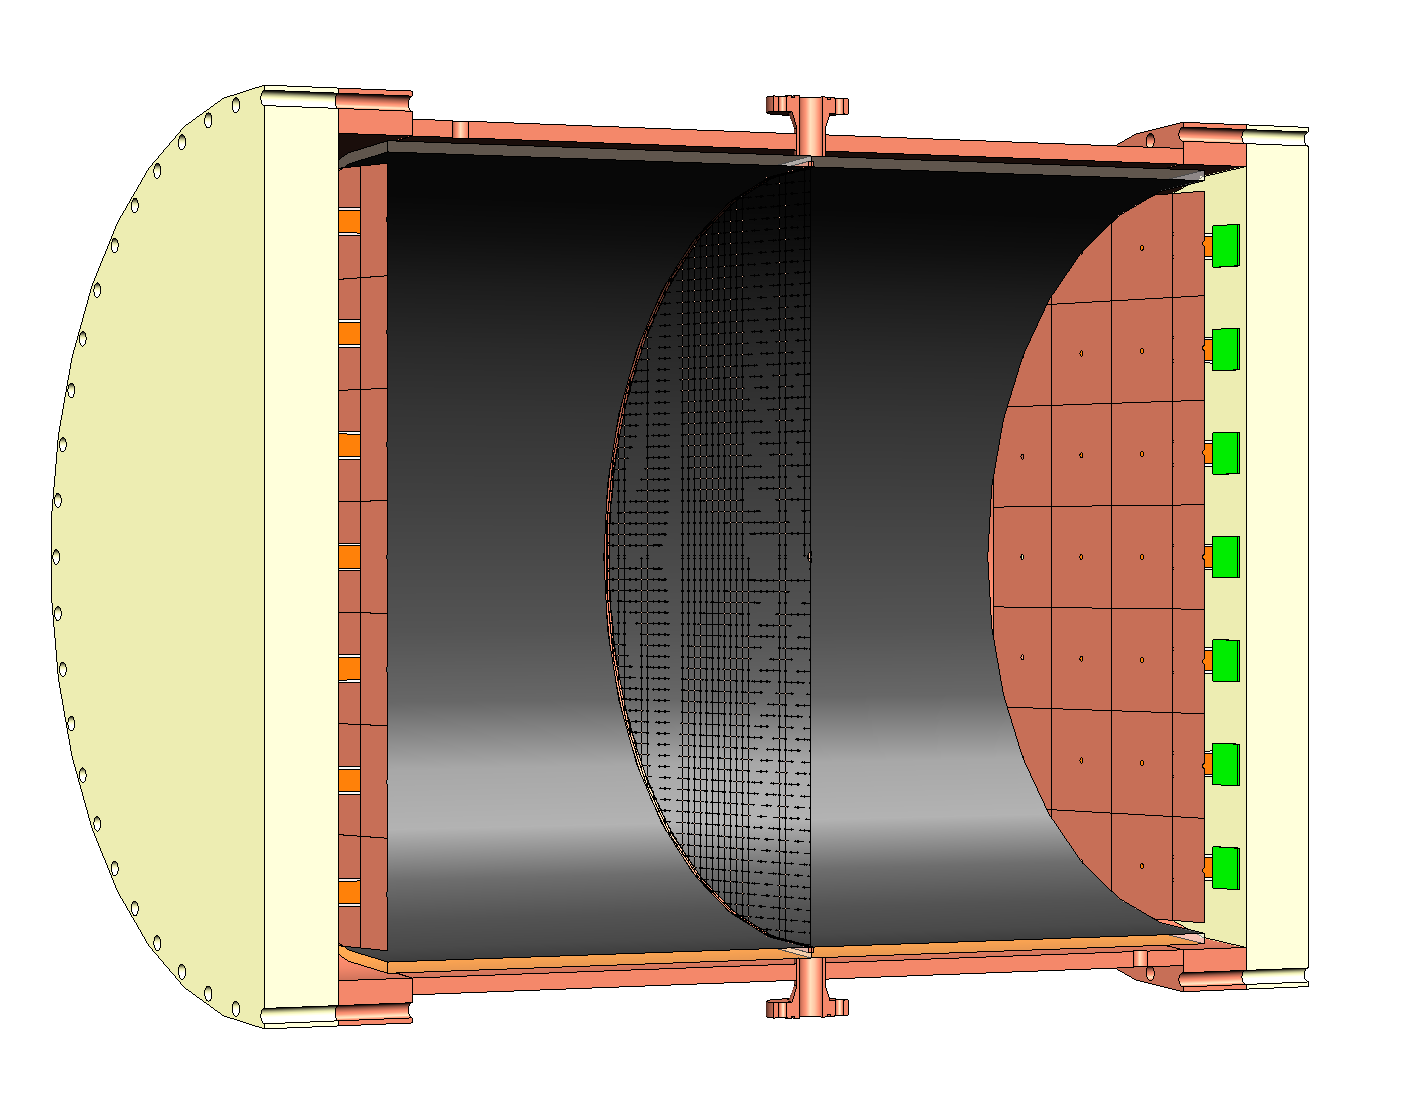
\includegraphics[width=0.4\columnwidth]{pic/fig1.png}
    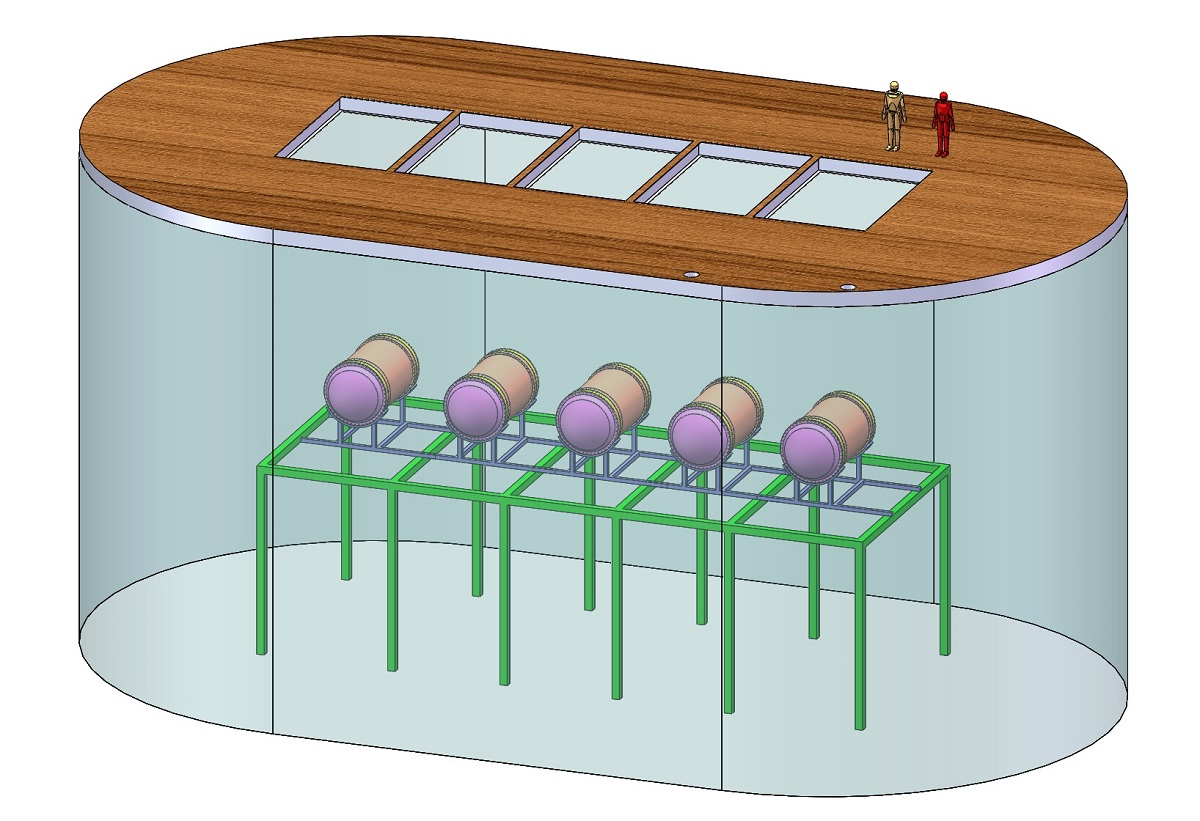
\includegraphics[width=0.4\columnwidth]{pic/fig2.jpg}
    \caption{左图:PandaX-III 实验中高压气氙 TPC 结构示意图。右图:放置在水池中的 5 个 TPC 所组成的 1 吨量级探测器示意图。\supercite{cdr}}
    \label{fig:detector}
\end{figure}
    
探测器主体是一个内高 2m,内直径 1.5m,使用高纯度无氧铜制作的柱形压力铜罐,总容积约为 3.5m$^3$。铜罐中心放置了圆形网状电极,内壁有等间隔的放置了 99 个圆形铜环,铜环之间以及铜环与内壁之间使用聚四氟乙烯(PTFE)隔离和支撑。这些铜环和极板共同组成一个场笼,为探测器提供了一个强度为 1kV/cm,延罐体轴心方向的漂移电场。铜罐壁厚度为 30mm,两端厚度为 150mm,放置于如\ref{fig:detector}右图所示的一个尺寸为 $27\times15\times13$m$^3$ 的水池中,利用超纯水来屏蔽周围环境的本底辐射。该水池建造在中国锦屏地下实验室中,利用实验室上方2500米厚的山岩屏蔽宇宙射线。对于探测器自身材料产生的本底辐射,PandaX-III 实验试图通过合理的探测器材料选择及结构设计来降低本底的数量。根据近年的研究,一些商业无氧铜材料中 \utte 和 \thttt 的含量可以低于0.1个 ppt(part per trillion)\supercite{abgrall2016majorana},是不锈钢材质的千分之一以上。本文在第\ref{chapter:background}章详细介绍了使用Geant4模拟分析得到的探测器本底事件组成。

\section{电子学以及读出}

为了提高探测器的能量分辨率,PandaX-III 实验使用了新型的被称作 Micromegas 的读出系统。它通过直接收集电离后的漂移电子来产生信号,结构简单,能量分辨率高,也容易控制自身材料带来污染。根据现有的针对 Microbulk Micromeags(一种 Micromegas,后称 MM)读出系统的详细研究,在 $Q_{\beta\beta}$ 附近使用它作为 10Bar Xe+TMA TCP 的读出,探测能够达到 3\% 的能量分辨率。PandaX-III 实验前期会直接向 CERN(European Organization for Nuclear Research,欧洲核子研究中心)订购 Microbulk Micromegas 成品,在实验的中后期则会尝试对读出系统做进一步的改进和优化以达到更佳的能量分辨率\supercite{cdr}。

在配合读出系统的电子学部件中,电子电气元器件很难做到放射性洁净,而且PCB板中的部分电路可能会游离出电子,为实验带来较大的背景污染。因此在探测器设计中,电子学部分被放置在铜罐两端外,使用 150mm 厚度的铜体来屏蔽它产生的背景辐射。同时为了能够重建出事件的径迹,读出系统需要做到像素读出或者是条状读出,为此所引入的大量通道数目也为电子学设计提出了挑战。PandaX-III 中期设计报告\supercite{cdr} 中详细描述了电子学以及数据获取系统的设计过程。

\section{PandaX-III实验设计总结及模拟工作}

为了探测寻找到NLDBD这样一极其稀有的事件,PandaX-III 实验在各个方面上都做了细致的考虑和设计,总结如下:

\vspace{0.4cm}

\begin{itemize}
    \item 提高探测器的灵敏度。
    \begin{itemize}
        \item 使用 10bar Xe+TMA 气体构建的 TPC 探测器。
        \item 使用新型 Microbulk MicroMegas 读出系统直接捕获漂移电子。
    \end{itemize}
    \item 减少本底辐射。
    \begin{itemize}
        \item 使用低本底材料构建探测器。
        \item 将探测器放置于中国锦屏地下实验室中的高纯水水池中,以此屏蔽宇宙射线以及环境中的本底辐射。
        \item 通过合理的探测器结构设计减少一些由材料带来的本底辐射。
    \end{itemize}
    \item 寻找合适的算法高效鉴别NLDBD信号和背景事件,以提高探测器的探测效率。
\end{itemize}

\vspace{0.4cm}

在这些设计的过程中,模拟工作发挥了相当的重要作用,它为整个实验提供了的数据支持。通过模拟我们可以测试不同设计时探测器灵敏度的差异,可以计算使用不同材料时本地辐射的变化,从而利用这些数据来指导探测器的设计。模拟工作也有助与读出系统及电子学的优化,为探测器标定的设计提供参考。在 PandaX-III 实验前期建造原型探测器验证的相关工作中,模拟数据可以验证测试结果,解释未知问题。可以说模拟工作是PandaX-III实验中相当重要的一环,本文在后续章节中详细介绍了这些模拟工作。

% vim:ts=4:sw=4
